\chapter{Special Relativity}
%TODO parts of chapter 1 and 2 that are not assigned yet
\section{Postulates and Definitions}
Special relativity is based on two main postulates, namely
\begin{enumerate}
    \item Principle of relativity: \\
    The laws of physics acquire the same form in all inertial systems.
    \item Constancy of the speed of light:\\
    The speed of light in vacuum is constant ${c\approx\unitfrac[3\cdot
    10^8]{m}{s}}$.
\end{enumerate}
We further define a series of objects, that will come handy when describing
relativity:
\begin{definition}[System of reference]
    A \emph{system of reference} $K$ is a system of three spacial coordinates
    to indicate the position and one time coordinate to indicate the time.
\end{definition}
\begin{definition}[Inertial system]
    An \emph{inertial system} $I$ belongs to a particular subspace of reference
    systems in which a freely moving bodies, i.e. that are not subject to any external
    force, move with constant velocity on an straight lines.
\end{definition}
\begin{definition}[Event]
    An \emph{event} or \emph{world point} $x$ is a point in spacetime. In any
    system of reference it can be described by four coordinates
    \begin{equation}
        x^\mu: (x^0,x^1,x^2,x^3)\, .
    \end{equation}
    For example in Cartesian coordinates, we have
    \begin{equation}
        (x^0,x^1,x^2,x^3) = (ct,x,y,z)\, .
    \end{equation}
\end{definition}
\begin{definition}[Worldline]
    A \emph{worldline} $\gamma$ is a parametrised curve in spacetime. To each
    parameter, there corresponds an event that lies on the worldline
    \begin{equation}
        \tensor{\gamma}{^\mu}(\lambda)=\tensor{x}{^\mu}(\lambda)\, .
    \end{equation}
\end{definition}
\subsection{Einstein Summation Convention}
Since we will have to deal which many indices, we will find a way to keep
notation as compact as possible. We agree that whenever we have a summation over an
upper and a lower index like $\sum_\mu \tensor{x}{_\mu}\tensor{x}{^\mu}$, we
drop the summation and assume that terms of type
$\tensor{x}{_\mu}\tensor{x}{^\mu}$ are always summed over.
\section{Propagation of Light Waves and the Line Element}
%For vividness, we restore factors of $c$ in this section.
%TODO picture
We consider the propagation of a light ray, characterized by two events $P$ and
$Q$, in an Inertial System $I$:
\begin{itemize}
    \item $P:$ Event of emission of the ray $(ct_1,x_1,y_1,z_1)$
    \item $Q:$ Event of absorption of the ray $(ct_2,x_2,y_2,z_2)$
\end{itemize}
The spatially distance between the events is
\begin{equation}
    r=\left[(x_2-x_1)^2+(y_2-y_1)^2+(z_2-z_1)^2\right]^{\frac{1}{2}}\, .
\end{equation}
Since we are tracking a light ray and the events are absorption and emission, we
further have
\begin{equation}
    r=c(t_2-t_1)\, .
\end{equation}
We construct the quantity
\begin{equation}
    {\Delta s}^2=-c^2(t_2-t_1)^2+(x_2-x_1)^2+(y_2-y_1)^2+(z_2-z_1)^2\, ,
\end{equation}
so that ${\Delta s}^2=0$ for light.

In another Inertial System $I'$, the events are given by
\begin{itemize}
    \item $P:$ Event of emission $(ct_1^\prime,x_1^\prime,y_1^\prime,z_1^\prime)$
    \item $Q:$ Event of absorption
    $(ct_2^\prime,x_2^\prime,y_2^\prime,z_2^\prime)$
\end{itemize}
By the same reasoning and the invariance of the physical laws and the
constancy of the speed of light, we have ${\Delta s^\prime}^2=0$ for light.
We define an infinitesimal interval, or \emph{line element}:
\begin{equation}
    \dif s^2=-c^2\dif t^2+\dif x^2+\dif y^2+\dif z^2\, .
\end{equation}
%TODO picture
Our preliminary considerations lead to the following statement: if the interval
is zero in one inertial system, it should be zero in all.
To relate the lineelements of different systems to each other, we make the
following thought:
Suppose we have three inertial Systems $I,I_1,I_2$.
The Systems $I_1$ and $I_2$ move at constant velocity $\vec{v}_1$ and $\vec{v}_2$ relative to $I$. Further
$I_2$ moves with velocity $\vec{v}_{12}$ relative to $I_1$. The demand implies
that there exists a function $\alpha$, only dependent on the velocity $\vec{v}$,
so that
\begin{equation}
    \dif s'^2=\alpha(\vec{v})\dif s^2\, .
\end{equation}
We have
\begin{equation}
    \dif s^2=\alpha(\vec{v}_1)\dif s_1^2\, ,\quad\dif s^2=\alpha(\vec{v}_2)\dif
    s_2^2\, ,\quad\dif s_1^2=\alpha(\vec{v}_{12})\dif s_2^2\, .
\end{equation}
Together they imply
\begin{equation}
    \alpha(\vec{v}_{12})=\frac{\alpha(\vec{v}_{2})}{\alpha(\vec{v}_{1})}\, ,
\end{equation}
but since the velocities where arbitary $\alpha$ has to be constant and we are
free to chose $\alpha\equiv 1$. Therefore the line element has to stay
invariant.
\section{Invariant Distances, Metric and Signature}
In flat space we can calculate the distance $\Delta l$ between two points
$(x_1,y_1)$ and $(x_2,y_2)$ by the \name{Pythagoras}' theorem
\begin{equation}
    \Delta l^2=\Delta x^2+\Delta y^2\, ,
    \quad \Delta x=x_2-x_1\,,\quad \Delta
    y=y_2-y_1\, .
\end{equation}
For an infinitesimal distance $\dif l$ we recover
\begin{equation}
    \dif l^2=\dif x^2+\dif y^2=\tensor{\delta}{_i_j}\dif x^i\dif x^j\, .
\end{equation}
If we introduce
\begin{equation}
    (\dif x^i)=\begin{bmatrix}
\dif x\\
\dif y
\end{bmatrix}\,,\quad (\delta_{ij})
=\begin{bmatrix}
1 & 0\\
0 & 1
\end{bmatrix}\, .
\end{equation}
We can expand the formula for the infinitesimal element and obtain
\begin{equation}
    \dif l^2=
    \begin{bmatrix}
        \dif x &
        \dif y
    \end{bmatrix}
    \begin{bmatrix}
        1 & 0\\
        0 & 1
    \end{bmatrix}
    \begin{bmatrix}
        \dif x\\
        \dif y
    \end{bmatrix}\, .
\end{equation}
Which we do to point out the similarity to the line element $\dif s^2$
\begin{equation}
    \dif s^2=
    \begin{bmatrix}
        \dif t &
        \dif x &
        \dif y &
        \dif z
    \end{bmatrix}
    \begin{bmatrix}
        -1 & 0 & 0 & 0\\
        0  & 1 & 0 & 0\\
        0  & 0 & 1 & 0\\
        0  & 0 & 0 & 1\\
    \end{bmatrix}
    \begin{bmatrix}
        \dif t\\
        \dif x\\
        \dif y\\
        \dif z\\
    \end{bmatrix}=:\eta_{\mu\nu}\dif x^\mu\dif x^\nu\, .
\end{equation}
We call the matrix $\eta_{\mu\nu}=\mathrm{diag}(-1,1,1,1)$ the
\emph{\name{Minkowski}-metric}. It has some obvious properties:
\begin{itemize}
    \item constancy: $\tensor{\eta}{_\mu_\nu_,_\varrho}=0$
    \item symmetry: $\tensor{\eta}{_\mu_\nu}=\tensor{\eta}{_\nu_\mu}$
    \item self inverse:
    $\tensor{\eta}{^\mu^\nu}:=\tensor{{\eta^{-1}}}{_\mu_\nu}=\tensor{\eta}{_\mu_\nu}$
\end{itemize}
We can use the metric to raise and lower indices:
\begin{equation}
    x_\nu=\tensor{\eta}{_\mu_\nu}x^\mu\, ,\quad x^\mu=\tensor{\eta}{^\mu^\nu}x_\nu\, .
\end{equation}
One has to pay attention with the matrix form, for example, the \emph{trace} of
the metric is given by
\begin{equation}
    \tensor{\eta}{^\mu_\mu}=\tensor{\eta}{^\mu^\nu}\tensor{\eta}{_\nu_\mu}
    =\tensor{\delta}{^\mu_\mu}=4\, .
\end{equation}
We say $\tensor{\eta}{_\mu_\nu}$ has signature $(-,+,+,+)$ or $(1,3)$, because
it has one negative and three positive eigenvalues.
\subsection{Poincaré-transformation}
To be consistent with a constant speed of light a transformation between two
coordinate systems must leave the line element invariant, i.e.
\begin{equation}
    \dif {s^\prime}^2 = \eta_{\mu\nu}\dif {x^\prime}^\mu\dif
    {x^\prime}^\nu=\eta_{\mu\nu}\dif x^\mu\dif
    x^\nu = \dif s^2\,. \label{eq:invarline}
\end{equation}
We consider afine coordinate transformations
\begin{equation}
    {x^\prime}^\mu= f^\mu(x^\nu)=\tensor{L}{^\mu_\nu}x^\nu+a^\mu\, .
\end{equation}
Where $\tensor{L}{^\mu_\nu}$ is a a \name{Lorentz} transformation and $a^\mu$
is a constant shift.\\
We can now inspect the transformation properties of an allowed transformation.
The invariance of the line element implies
\begin{equation}
    \dif {s^\prime}^2 = \eta_{\mu\nu}\dif {x^\prime}^\mu\dif
    {x^\prime}^\nu=\eta_{\varrho\sigma}\tensor{L}{^\varrho_\mu}\tensor{L}{^\sigma_\nu}\dif
    x^\mu\dif x^\nu \stackrel{!}{=} \dif s^2\,,
\end{equation}
independent of the shift $a^\mu$. We will therefore focus our attention towards
the linear transformation $\tensor{L}{^\mu_\nu}$. Equation
\eqref{eq:invarline} implies that
\begin{equation}
    \eta_{\mu\nu}=\tensor{L}{^\varrho_\nu}\eta_{\varrho\sigma}\tensor{L}{^\sigma_\nu}\,.\label{eq:invariance}
\end{equation}
We can take a look at an infinitimal transformation, that is up to an order of
$\varepsilon^2$
\begin{equation}
    \tensor{L}{^\mu_\nu}=\tensor{\delta}{^\mu_\nu}
    +\varepsilon\tensor{\omega}{^\mu_\nu}\, .
\end{equation}
The $\tensor{\omega}{^\mu_\nu}$ are called the \emph{generators} of the
transformation. Plugging into \eqref{eq:invariance}, ignoring higher powers in
$\varepsilon^2$ results in
\begin{equation}
    \begin{split}
        \eta_{\mu\nu}&=\eta_{\varrho\sigma}\left(\tensor{\delta}{^\varrho_\mu}
        +\varepsilon\tensor{\omega}{^\varrho_\mu}\right)\left(\tensor{\delta}{^\sigma_\nu}
        +\varepsilon\tensor{\omega}{^\sigma_\nu}\right)\\
        &=
        \eta_{\mu\nu}+\varepsilon\left(\tensor{\omega}{_\mu_\nu}+\tensor{\omega}{_\nu_\mu}\right)\,
        .
    \end{split}
\end{equation}
Since this must hold true for arbitrary $\varepsilon$, the generators
$\tensor{\omega}{_\nu_\mu}$ must satisfy
$\tensor{\omega}{_\nu_\mu}=-\tensor{\omega}{_\mu_\nu}$, i.e. be antisymmetric.
In general we have $\frac{n(n-1)}{2}$ of these objects, where $n$ is the
dimension of the underlying space.
Since we are considering four dimensional spacetime, there are six generators.
The finite transformations by an generalized angle $\alpha\in\Complex$ can be
obtained from the generators via
\begin{equation}
    \tensor{L}{^\mu_\nu}=\exp\left(\alpha\tensor{\omega}{^\mu_\nu}\right)\,.
\end{equation}
We can
classify the resulting transformations into two classes:
\subsubsection{Rotations}
Rotations mix the spatial coordinates, but leave the time fixed. Consider for
example an rotation around $z$-axis. Then we have
\begin{equation}
    x^\prime=x\cos\alpha+y\sin\alpha \, ,\quad y^\prime=-x\sin\alpha+y\cos\alpha \, .
\end{equation}
The infinitesimal generator is
\begin{equation}
    \tensor{\omega}{^\mu_\nu}
    =
    \begin{bmatrix}
        0&0 & 0&0\\
        0&0 &1&0\\
        0&-1&0 &0\\
        0&0 &0 &0
    \end{bmatrix}\,
\end{equation}
and the transformation can be expressed in matrix form
\begin{equation}
    \begin{bmatrix}
        t\\
        x\\
        y\\
        z\\
    \end{bmatrix}=
    \begin{bmatrix}
        1&0 & 0&0\\
        0&\cos\alpha &\sin\alpha&0\\
        0&-\sin\alpha&\cos\alpha &0\\
        0&0 &0 &1
    \end{bmatrix}
    \begin{bmatrix}
        t^\prime\\
        x^\prime\\
        y^\prime\\
        z^\prime
    \end{bmatrix}
\end{equation}
\subsubsection*{Boosts}
Boosts can be thought of as rotations between time and spacial coordinates. We
consider a boost in $x$-direction. Since the line element must be invariant and
a linear transformation keeps the origin fixed we have
\begin{equation}
    -t^2+x^2=-{t^\prime}^2+{x^\prime}^2\, .
\end{equation}
This is an hyperbolic equation and can be parametrised by
\begin{equation}
    t = t^\prime\cosh\psi+x^\prime\sinh\psi\,, \quad x =
    t^\prime\sinh\psi+x^\prime\cosh\psi\, .
\end{equation}
Where $\psi$ is called the \emph{rapidity}.
The generator is
\begin{equation}
    \tensor{\omega}{^\mu_\nu}
    =
    \begin{bmatrix}
        0&1 & 0&0\\
        1&0 &0&0\\
        0&0&0 &0\\
        0&0 &0 &0
    \end{bmatrix}\,.
\end{equation}
The matrix form of the transformation is
\begin{equation}
    \begin{bmatrix}
        t\\
        x\\
        y\\
        z\\
    \end{bmatrix}=
    \begin{bmatrix}
        \cosh\psi&\sinh\psi & 0&0\\
        \sinh\psi&\cosh\psi &0&0\\
        0&0&1 &0\\
        0&0 &0 &1
    \end{bmatrix}
    \begin{bmatrix}
        t^\prime\\
        x^\prime\\
        y^\prime\\
        z^\prime
    \end{bmatrix}\, .
\end{equation}
The rapidity $\psi$ is not related to a physical quantity yet. We may ask to
which velocity $v$ does this boost correspond.
Therefore we consider the line $x^\prime= 0$.
Then
\begin{equation}
    t=t^\prime\cosh\psi\, ,\quad
    x=t^\prime\sinh\psi\, .
\end{equation}
We can express the velocity $v$, as seen by an observer in the primed system
\begin{equation}
    v=\frac{x}{t}=\tanh\psi\,.
\end{equation}
It is convenient to introduce the parameters $\beta$ and $\gamma$ defined as
follows
\begin{equation}
    \beta:=v\, ,\quad\gamma:=\frac{1}{\sqrt{1-\beta^2}}\, .
\end{equation}
In terms of these we find
\begin{equation}
    \sinh\psi = \beta\gamma\, , \quad \cosh\psi=\gamma\,.
\end{equation}
Therefore an alternative form is given by
\begin{equation}
    \tensor{L}{^\mu_\nu}=\begin{bmatrix}
\gamma&\beta\gamma & 0&0\\
\beta\gamma&\gamma &0&0\\
0&0&1 &0\\
0&0 &0 &1
\end{bmatrix}\, .
\end{equation}
And the coordinates are therefore related by
\begin{equation}
    t=\gamma\left(t^\prime+\beta x^\prime\right)\,,\quad
    x=\gamma\left(x^\prime+\beta t^\prime\right)\, .
\end{equation}
All together we have ten independent (affine) transformations that leave the
line element invariant. Namely:
\begin{itemize}
    \item four shifts by $a^\mu=(a^0,a^1,a^2,a^3)\transpose$
    \item three rotations in space corresponding to three real angles
    $\boldsymbol{\theta}=(\theta_1,\theta_2,\theta_3)\transpose$ (Euler angles)
    \item three boosts with constant velocity $\vec{v}=(v_1,v_2,v_3)\transpose$
\end{itemize}
The \name{Poincaré} transformations form a ten parameter group.
\begin{table}
    \centering
    \caption{Comparison of \name{Newton}ian theory and special relativity.}
    \begin{tabulars}{lll}
        \toprule
        &\name{Newton}&\name{Einstein} (SR)\\
        \midrule
        & law of inertia
        & law of inertia \\
        \name{Newton}'s Laws
        & $\vec{F}=m\ddot{\vec{x}}=m\od{\vec{p}}{t}$
        &$\vec{F}=m\od{\vec{p}}{\tau}$\\
        & $\vec{F}_{12}=-\vec{F}_{21}$
        & momentum conservation\\
        &
        &(postulate)\\
        transformations
        & \name{Poincaré} transformations
        & \name{Galilei} transformations\\
        
        & absolute structure
        & absolute time\\
        
        & $c=\mathrm{const.}$
        & $t^\prime=t$\\
        force
        &$\vec{F}=\frac{G\textsubscript{N}m_1m_2}{r^2}$
        &$F^\alpha= \frac{q}{m} U_\beta
        \tensor{F}{^\alpha^\beta}$,\,  $F
        =\gamma(f_0,\vec{f})\transpose$\\
        &$\Delta \Phi =4\pi\varrho$ &\name{Maxwell}'s equations
        \\
        \bottomrule
    \end{tabulars}
\end{table}

\section{Vectors and Tensors in SRT}
%TODO connect subsections
At this point we will just list some objects, that we call vectors and tensors
and delay the definition of those to a later chapter.
A bit sloppy we refer to a vector $V$ with components $\tensor{V}{^\mu}$, as a
object that transforms as
\begin{equation}
    \tensor{V}{^\mu}\to
    \tensor{L}{^\mu_\alpha}\tensor{V}{^\alpha}\,
\end{equation}
and to a tensor as a 'vector with more indices' that
transforms accordingly, i.e.
\begin{equation}
    \tensor{T}{^\mu^\nu}\to
    \tensor{L}{^\mu_\alpha}\tensor{L}{^\nu_\beta}\tensor{T}{^\alpha^\beta}\,,
\end{equation}
and so forth.
An example of a vector is the four current $J^\mu$:
\begin{equation}
    J^\mu=\gamma(\varrho,\vec{j})\transpose\, ,
\end{equation}
with $\varrho$ the charge density and $\vec{j}$ the 3-current density.
A typical example is the field strength tensor
$\tensor{F}{^\mu^\nu}$ of electrodynamics given in terms of the
vector potential $\tensor{A}{_\mu}$:
\begin{equation}
    \tensor{F}{_\mu_\nu}=\partial_\mu\tensor{A}{_\nu}-\partial_\nu\tensor{A}{_\mu}\,.
\end{equation}
The matrix form is
\begin{equation}
    \tensor{F}{_\mu_\nu}=
    \begin{bmatrix}
        0  &   E_1 &  E_2 &  E_3 \\
        -E_1 &   0  &  -B_3 & B_2 \\
        -E_2 & B_3 &   0  &  -B_1 \\
        -E_3 &  -B_2 & B_1 &   0  \\
    \end{bmatrix}\, .
\end{equation}
Therefore the tensor $\tensor{F}{^\mu^\nu}$ takes the role of the fields
$\vec{E},\vec{B}$. In tensor form \name{Maxwell} equations take the particular
simple form, namely
\begin{equation}
    \label{eq:maxwell_eqs}
    \partial_\nu\tensor{F}{^\mu^\nu}=4\pi\tensor{J}{^\mu}\,, \quad
    \partial_\alpha\tensor{F}{_\mu_\nu}
    +\partial_\nu\tensor{F}{_\alpha_\mu}
    +\partial_\mu\tensor{F}{_\nu_\alpha}=0\,.
\end{equation}
The \name{Lorentz} force is given by
\begin{equation}
    \tensor{F}{^\mu}=q\tensor{F}{^\mu^\nu}\tensor{u}{_\nu}
\end{equation}
Where $\tensor{u}{^\mu}=\gamma(1,\vec{v})\transpose$ is the four velocity. As
another example we can take a look at plane waves. The vector potential of a plane wave is
\begin{equation}
    \tensor{A}{^\mu}=\tensor{\hat{A}}{^\mu}
    \exp\left[\imI(\vec{k}\cdot\vec{r}-\omega
    t)\right]
    =\tensor{\hat{A}}{^\mu}\exp\left(\imI\tensor{K}{^\mu} \tensor{X}{_\mu}\right)\,
    .
\end{equation}
Where $\tensor{K}{^\mu}=\left(\omega,\vec{k}\right)\transpose$ must be a four
vector, because otherwise we could use plane waves to distinguish between
inertial systems. The dispersion relation reads as
\begin{equation}
    \tensor{K}{^\mu}\tensor{K}{_\mu}=-\omega^2+\vec{k}^2=0\, .
\end{equation}
It is equivalent to the on shell condition \eqref{eq:onshell}, when we identify
the photons energy $E=\omega$, momentum $\vec{p}=\vec{k}$ and mass $m=0$.
\subsection{Fourvectors}
There are three types of vectors\footnote{We could also put up a fourth class,
containing solely the zero vector.}:
\begin{enumerate}
    \item \emph{spacelike} $\Delta\tensor{x}{^\mu}\Delta\tensor{x}{_\mu}>0$
    \item \emph{lightlike} $\Delta\tensor{x}{^\mu}\Delta\tensor{x}{_\mu}=0$
    \item \emph{timelike} $\Delta\tensor{x}{^\mu}\Delta\tensor{x}{_\mu}<0$
\end{enumerate}
All classes are transformed into themselves by \name{Lorentz} transformation.
There is a set of transformations that is forbidden by physical considerations: namely the
parity change $\vec{x}\to -\vec{x}$ and time reversal $t\to -t$ because this are
no real symmetries of nature\footnote{both violated in weak interactions.}.
We will mainly deal with timelike and lightlike vectors for which the time order
does not change. For spacelike intervals the order can change. To remain causal
all particles have to move at velocity $v\leq c$. This is in contrast to
Newtonian theory where everything can affect everything, because the velocities
are unbounded. A direct consequence of this is for example that even the two
body problem has no exact solution in special relativity.
Tabular~\ref{tab:fourvecs} shows a list of the dynamic fourvectors in SR,
notice that in contrast to the classical, theory the fouraccelaration
$\tensor{a}{_\mu}$ has no importance in SR.
\begin{table}
    \centering
    \caption{Examples of fourvectors and normalisation.\label{tab:fourvecs}}
    \begin{tabulars}{lll}
        \toprule
        fourvector&definition&normalisation\\
        \midrule
        velocity
        &$\tensor{u}{^\mu}=\od{\tensor{x}{^\mu}}{\tau}=\gamma(1,\vec{v})\transpose$
        &$\tensor{u}{_\mu}\tensor{u}{^\mu}=-1$\\
        momentum
        &$\tensor{p}{^\mu}:=m\tensor{u}{^\mu}$
        &$\tensor{p}{_\mu}\tensor{p}{^\mu}=-m^2$\\
        acceleration&$\tensor{a}{^\mu}:=\od{\tensor{u}{^\mu}}{\tau}$&$\tensor{a}{_\mu}\tensor{a}{^\mu}=0$\\
        \bottomrule
    \end{tabulars}
\end{table}
\subsection{The Energy Momentum Tensor}
%TODO consider using different source.
%TODO consider merging with The Energy Momentum Tensor
\begin{sidenote}
Above a certain limit a, system cannot be stabilized by pressure, because the
gravity couples to the pressure and therefore increasing the pressure would lead
to a stronger attraction due to gravity and hence unfetchable collapse.
\end{sidenote}
%TODO sidenote does not fit context
The energy momentum tensor is symmetric
\begin{equation}
    \tensor{T}{^\mu^\nu}=\tensor{T}{^\nu^\mu}\, .
\end{equation}
Its trace is given by
\begin{equation}
    \tensor{T}{^\mu_\mu}=(\varrho-p)+4p=-\varrho+3p\, .
\end{equation}
It is traceless for photons. If an external field is present the divergence is
given by
\begin{equation}
    \tensor{T}{^\mu^\nu_,_\nu}=\tensor{D}{^\mu}\,  .
\end{equation}
Where the external momentum is itself given as the divergence
\begin{equation}
    \tensor{D}{^\mu} =-\tensor{S}{^\mu^\nu_,_\nu}\, .
\end{equation}
Putting both terms together gives
\begin{equation}
    \partial_\mu(\tensor{T}{^\mu^\nu}+\tensor{S}{^\mu^\nu})=0\,,
\end{equation}
Which can be interpreted as the total energy conservation.
\subsection{Noether's Theorem}
We introduce a tensorial generalisation of the angular momentum
\begin{equation}
    \tensor{T}{^\lambda^\mu^\nu}:=
    \tensor{x}{^\lambda}\tensor{T}{^\mu^\nu}-\tensor{x}{^\mu}\tensor{T}{^\lambda^\nu}\,
    .
\end{equation}
The angular momentum is given by
\begin{equation}
    \tensor{L}{^i^j} = \int\dif{}^3 x \tensor{M}{^i^j^0}\, .
\end{equation}
%TODO what doe the components mean
It can be shown that it is a conserved quantity
\begin{equation}
    \tensor{\partial}{_\nu}\left(\tensor{x}{^\lambda}\tensor{T}{^\mu^\nu}-\tensor{x}{^\nu}\tensor{T}{^\lambda^\nu}\right)
    =\tensor{T}{^\mu^\lambda}-\tensor{T}{^\lambda^\mu}+\tensor{x}{^\lambda}
    \tensor{T}{^\mu^\nu_,_\nu}-\tensor{x}{^\nu}\tensor{T}{^\lambda^\nu_,_\nu}=0\, .
\end{equation}
\begin{remark}
The existence of a conserved symmetric tensor $\tensor{T}{^\mu^\nu}$ is
necessary in order to build a relativistic theory
\end{remark}
\begin{example}[Electrodynamics]
We start by inspecting the \name{Lorentz} Force $\tensor{F}{^\mu}$ which is
given by
\begin{equation}
    \tensor{F}{^\mu}=e\tensor{F}{^\mu^\nu}\tensor{u}{_\nu}=\tensor{F}{^\mu^\nu}\tensor{J}{_\nu}=\tensor{D}{^\mu}\,
    .
\end{equation}
We now ask whether there is a potential $\tensor{S}{^\mu^\nu}$ so that
$\tensor{D}{^\mu}=-\tensor{S}{^\mu^\nu_{,\nu}}$. Indeed a potential is given by
\begin{equation}
    \tensor{S}{^\mu^\nu}=\tensor{F}{^\mu_\alpha}\tensor{F}{^\nu^\alpha}-\frac{1}{4}\tensor{\eta}{^\mu^\nu}\tensor{F}{_\alpha_\beta}\tensor{F}{^\alpha^\beta}\,
    .
\end{equation}
We can check
\begin{equation}
    \tensor{S}{^\mu^\nu_{,\nu}}=\tensor{F}{^\mu_\alpha_{,\nu}}\tensor{F}{^\nu^\alpha}+
    \tensor{F}{^\mu_\alpha}\tensor{F}{^\nu^\alpha_{,\nu}}
    -\frac{1}{2}\tensor{\eta}{^\mu^\nu}\tensor{F}{_\alpha_\beta_{,\nu}}\tensor{F}{^\alpha^\beta}\,
    .
\end{equation}
\begin{align}
    \tensor{F}{^\mu_\alpha_{,\nu}}\tensor{F}{^\nu^\alpha}
    &=\tensor{F}{^\mu_\nu_{,\alpha}}\tensor{F}{^\alpha^\nu}
    =\tensor{F}{^\nu_\mu_{,\alpha}}\tensor{F}{^\nu^\alpha}
    \\
    %\tensor{F}{^\mu_\alpha}\tensor{F}{^\nu^\alpha_{,\nu}}&=\\
    \tensor{\eta}{^\mu^\nu}\tensor{F}{_\alpha_\beta_{,\nu}}\tensor{F}{^\alpha^\beta}
    &=\tensor{F}{_\alpha_\nu^{,\mu}}\tensor{F}{^\alpha^\nu}
    = -\tensor{F}{_\alpha_\nu^{,\mu}}\tensor{F}{^\nu^\alpha}
    \,
    .
\end{align}
%TODO calculation
\begin{equation}
    \tensor{S}{^\mu^\nu_{,\nu}}=\tensor{F}{^\nu_\mu_{,\alpha}}\tensor{F}{^\nu^\alpha}
    +\frac{1}{2}\tensor{F}{_\alpha_\nu^{,\mu}}\tensor{F}{^\nu^\alpha}
\end{equation}
The Lagrangian of electrodynamics is given by
\begin{equation}
    \mathcal{L}=-\frac{1}{2}\tensor{F}{_\mu_\nu}\tensor{F}{^\mu^\nu}+\tensor{J}{_\mu}\tensor{A}{^\mu}-\frac{1}{2}m^2\tensor{A}{_\mu}\tensor{A}{^\mu}\,
    .
\end{equation}
The tensor $S$ is known as \emph{electromagnetic stress–energy tensor} and
given in contravariant form as
\begin{equation}
    \tensor{S}{^\mu^\nu}=
    \begin{pmatrix}
        u&\vec{S}\transpose\\
        \vec{S}& -\tensor{\sigma}{_i_j}
    \end{pmatrix}\,.
\end{equation}
Where
$\tensor{\sigma}{_i_j}=\tensor{E}{_i}\tensor{E}{_j}+\tensor{E}{_i}\tensor{E}{_j}-\frac{1}{2}\tensor{\delta}{_i_j}\left(\vec{E}^2+\vec{B}^2\right)$
is the \emph{\name{Maxwell} stress tensor}, $\vec{S}=\vec{E}\times\vec{B}$
\emph{\name{Poynting} vector} and energy density $u
=\frac{1}{2}\left(\vec{E}^2+\vec{B}^2\right)$.
\end{example}

\section{Lagrangian Formalism}
We want to formulate special relativity in terms of a variation principle.
Therefore we consider massive particles, i.e. timelike paths. As a postulate we
take that the action $S$ is proportional to the proper time (as a generalized
``distance'') $\dif \tau:=\sqrt{-\dif s^2}$
\begin{equation}
    S= -\alpha \int_a^b\dif \tau = -\alpha
    \int_{t_1}^{t^2}\sqrt{1-\vec{v}^2}\dif t =: \int_{t_1}^{t^2}L\dif t\, ,
\end{equation}
with $\alpha$ a constant, that has to be determined. The Lagrangian $L$ is
given by
\begin{equation}
    L=-\alpha\sqrt{1-\vec{v}^2}\simeq
    -\alpha\left(1-\frac{1}{2}\vec{v}^2+\ldots\right) \, .
\end{equation}
We demand that we recover the classical theory in the limit $\vec{v}\to 0$. The
the lowest order kinetic term is
\begin{equation}
    T=\frac{1}{2}\alpha \vec{v}^2\, .
\end{equation}
Comparing with the classical kinetic energy $T=\frac{1}{2}m\vec{v}^2$ yields
$\alpha=m$. If we substitute $\alpha$ we recover the Lagrangian of
special relativity
\begin{equation}
    L\textsubscript{SR}=-m\sqrt{1-\vec{v}^2}=-m\gamma^{-1}\, .
\end{equation}
We can proceed calculate the generalized momenta
\begin{equation}
    p_i=\dpd{L}{v_i}=\frac{mv_i}{\sqrt{1-\vec{v}^2}}=\gamma m v_i\, .
\end{equation}
The energy can be calculated via the Hamiltonian $H$
\begin{equation}
    E=H=\vec{p}\cdot\vec{v}-L=\gamma m \vec{v}^2 + m\gamma^{-1} =\gamma m\, .
\end{equation}
Expanded in $\vec{v}^2$ the energy reads as
\begin{equation}
    E=m+\frac{1}{2}m\vec{v}^2+\ldots\, .
\end{equation}
If we restore units of $c$ for a moment we get that the constant term is
equal to $mc^2$. This is \name{Einstein}'s famous $E=mc^2$.
We can further relate energy and momentum to each other. Therefore consider the
square of the momentum $\vec{p}$
\begin{equation}
    \vec{p}^2=\frac{m\vec{v}^2}{1-\vec{v}^2}\, .
\end{equation}
Solving for $\vec{v}^2$ yields
\begin{equation}
    \vec{v}^2=\frac{\vec{p}^2}{\vec{p}^2+m^2}\, .
\end{equation}
Which we can insert in the expression for the energy
\begin{equation}
    E^2=\frac{m^2}{1-\vec{v}^2}=\vec{p}^2+m^2 \label{eq:onshell}\, .
\end{equation}
The equation \eqref{eq:onshell} is called the \emph{on shell condition}.
\begin{figure}
\centering
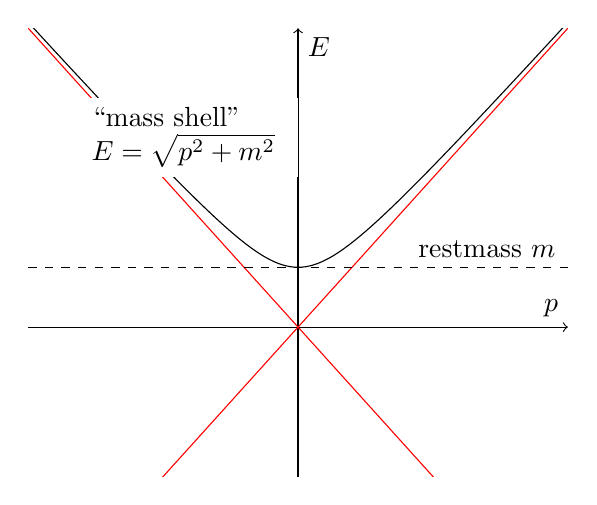
\begin{tikzpicture}
  \begin{axis}[
    xmin=-10,xmax=10,
    ymin=-5,ymax=10,
    xlabel={$p$},
    ylabel={$E$},
    xtick={0},
    ytick={0},
    xticklabels={,,},
    yticklabels={,,},
    axis lines=center,
    axis line style=->]
    \addplot[] expression[domain=-10:10,samples=100]{(4+x^2)^(1/2)}; 
    \addplot[red] expression[domain=-10:10,samples=100]{x}; 
    \addplot[red] expression[domain=-10:10,samples=100]{-x}; 
    \addplot[dashed] expression[domain=-10:10,samples=100]{2}; 
    \pgfplotsset{
    after end axis/.code={
        \node[above] at (axis cs:7,2){restmass $m$};
        \node[above,text width=2.5cm,fill=white] at (axis cs:-4,5){``mass shell''\\$E=\sqrt{p^2+m^2}$};
    }
}
  \end{axis}
\end{tikzpicture}
\caption{Energy $E$ of a particle with mass $m$, as a function of the momentum
$p$.}
\end{figure}


\begin{sidenote}[On massive photons]
There is nothing in the theory that predicts that the photon is massless. It
could be possible that its mass is only really small and that in fact that the
photon does not travel at the speed of light. (Of course this would make it
convenient to rename the constant $c$) Even though the mass should be so small
that the de Broglie wavelength is of the order of the size of the universe,
massive photons would have a huge impact.
\end{sidenote}
\begin{sidenote}[Complex Time]
We could in principle make a substitution $t\to \imI t$. Which would free us
from the need to distinguish between co- and contravariant vectors, because the
inner product would be given as
\begin{equation}
    g(x,y)=\left(\imI x^0\right)\left(\imI
    y^0\right)+\vec{x}\cdot\vec{y}=-x^0y^0+\vec{x}\cdot\vec{y}
\end{equation}
and hence $\tensor{g}{_i_j}=\tensor{\delta}{_i_j}$, which basically means we can
raise and lower indices at will. This is practical whenever you do calculations,
e.g. in computer simulations.
\end{sidenote}
